\chapter{Verification \& Validation}
\label{chap:v_and_v}
\graphicspath{{V&V/}}

In this chapter, we will present the results on verification and validation of the simulator discussed in \Cref{chap:naos}. We verify the gravity model, the launch conditions for the regolith, the numerical integrator along with the equations of motion for the regolith, and finally the Solar perturbation models. We validate our simulator to ensure that our inferences for any scientific result out of it remains true and valid as well.

\section{Constant Density Ellipsoid Gravity Model}
\label{sec:gravity_vv}
The \gls{CDE} gravity model was tested for a singular target point by comparing the gravitational potential and acceleration values at that point as computed by \gls{NAOS}, with external data obtained from another researcher at CSML \footnote{Centre for Spaceflight Mechanics Laboratory; The thesis work was partly done at CSML, which is a research lab headed by Dr. Daniel Scheeres and is part of the University of Colorado, Boulder, USA.}. The parameters used for the test are given in \Cref{tab:gravity_vv_params}.
%%%
\begin{table}[htb]
\centering
\captionsetup{justification=centering}
\caption{Parametric values used for testing the \gls{CDE} gravitational potential model.}
\label{tab:gravity_vv_params}
\begin{tabular}{|l|l|l|}
\hline
\multicolumn{1}{|c|}{\textbf{Parameter}} & \multicolumn{1}{c|}{\textbf{Value}} & \multicolumn{1}{c|}{\textbf{Units}}      \\ \hline
Gravitational Parameter                  & 446382.0                            & \si{\metre \cubed \per \second \squared} \\ \hline
Alpha (longest axis of \gls{CDE})      & 20000                               & \si{\metre}                            \\ \hline
Beta (Intermediate axis of \gls{CDE})  & 7000                                & \si{\metre}                            \\ \hline
Gamma (Shortest axis of \gls{CDE})     & 7000                                & \si{\metre}                            \\ \hline
Target point x-coordinate                & 10000                               & \si{\metre}                            \\ \hline
Target point y-coordinate                & 13000                               & \si{\metre}                            \\ \hline
Target point z-coordinate                & 8000                                & \si{\metre}                            \\ \hline
\end{tabular}
\end{table}
\FloatBarrier
%%%
The test values for the gravitational potential and the acceleration values at the specified target point are given in \Cref{tab:gravity_vv_test_values}.
%%%
% Please add the following required packages to your document preamble:
% \usepackage{multirow}
\begin{table}[htb]
\centering
\captionsetup{justification=centering}
\caption{Test values for verification of the \gls{CDE} gravity model.}
\label{tab:gravity_vv_test_values}
\begin{tabular}{|l|l|l|l|}
\hline
\multicolumn{1}{|c|}{\textbf{Parameter}}    & \multicolumn{2}{c|}{\textbf{Value}}     & \multicolumn{1}{c|}{\textbf{Units}}          \\ \hline
Gravitational Potential                     & \multicolumn{2}{l|}{23.710052554396402} & \si{\metre \squared \per \second \squared} \\ \hline
\multirow{3}{*}{Gravitational Acceleration} & x       & -0.00044762916738340803       & \si{\metre \per \second \squared}          \\ \cline{2-4}
                                            & y       & -0.0009623388813999501        & \si{\metre\per \second \squared}           \\ \cline{2-4}
                                            & z       & -0.000592208542399969         & \si{\metre\per \second \squared}           \\ \hline
\end{tabular}
\end{table}
\FloatBarrier
%%%
The values obtained from the simulator \gls{NAOS} were compared with the ones in \Cref{tab:gravity_vv_test_values} upto the 12th decimal point and they matched, validating the gravity model implemented in \gls{NAOS}.

\section{Regolith Launch Conditions}
\label{sec:regolith_launch_conditions_vv}
In this section, we'll presents results on verifying whether the initial state vector for the regolith or the launch condition match to what is desired by the user. Here, an internal validation is done to ensure that the launch conditions registered in the output database match the raw value input to \gls{NAOS}. We present graphical and numerical results in this regard.

\subsection{Launch Location}
\label{subsec:launch_location_vv}
The position vector to the launch location, from the centre of the \gls{ARF}, is formed by giving only the launch location latitude and longitude as input. Thus, we have to verify whether the position vector conforms to a given angular input. We take the initial state vector, from the output databases of the dynamics simulator, of regolith launched from a few launch locations on the asteroid and convert the Cartesian coordinates back to latitude and longitude to see if the position vector was formed correctly. For the same Cartesian coordinates, we use the triaxial ellipsoid equation, and see if they solve the equation, to verify that the launch point lies on the surface of the asteroid.
%
\newline\newline
%
We took 5 test locations from where regolith was launched and separately calculated the corresponding longitude and latitude for the launch location to check if the position vector was correctly formed. The position coordinates and the back-calculated latitude and longitude angles are shown in \Cref{tab:position_vector_to_lat_long_vv}.
%%%
\begin{table}[htb]
\centering
\captionsetup{justification=centering}
\caption{Position vector to different launch locations and the corresponding Latitude and Longitude angles.}
\label{tab:position_vector_to_lat_long_vv}
\begin{tabular}{|c|c|c|c|c|}
\hline
\textbf{X {[}m{]}} & \textbf{Y {[}m{]}} & \textbf{Z {[}m{]}} & \textbf{Longitude {[}deg{]}} & \textbf{Latitude {[}deg{]}} \\ \hline
20000.0 & 0.0 & 0.0 & 0.0 & 0.0 \\ \hline
0.0 & 7000.0 & 0.0 & 90.0 & 0.0 \\ \hline
0.0 & 0.0 & 7000.0 & 0.0 & 90.0 \\ \hline
3316.14545023 & 1914.57746836 & 6632.29090046 & 30.0 & 60.0 \\ \hline
-3961.38284482 & -3961.38284482 & 5602.2413449 & -135.0 (225.0) & 45.0 \\ \hline
\end{tabular}
\end{table}
\FloatBarrier
%%%
The longitude and latitude values given in \Cref{tab:position_vector_to_lat_long_vv} were calculated from the Cartesian coordinates and match those given as inputs to the dynamics simulator. The position vectors from \Cref{tab:position_vector_to_lat_long_vv} with the \gls{CDE} model are also depicted in \Cref{fig:position_vector_diagram}.
%%%
\begin{figure}[htb]
\centering
\captionsetup{justification=centering}
\subfloat[]{
    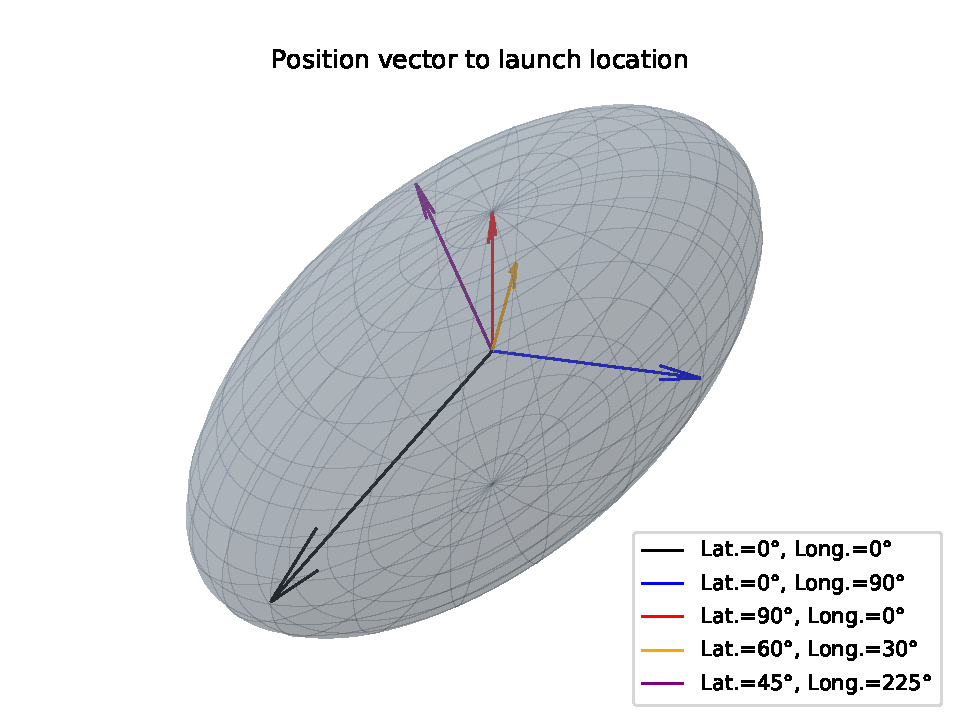
\includegraphics[width=\textwidth, height=0.4\textheight, keepaspectratio=true]{Images/launch_location_position_vectors.pdf}
    \label{fig:launch_location_vv_1}
    }

\subfloat[]{
    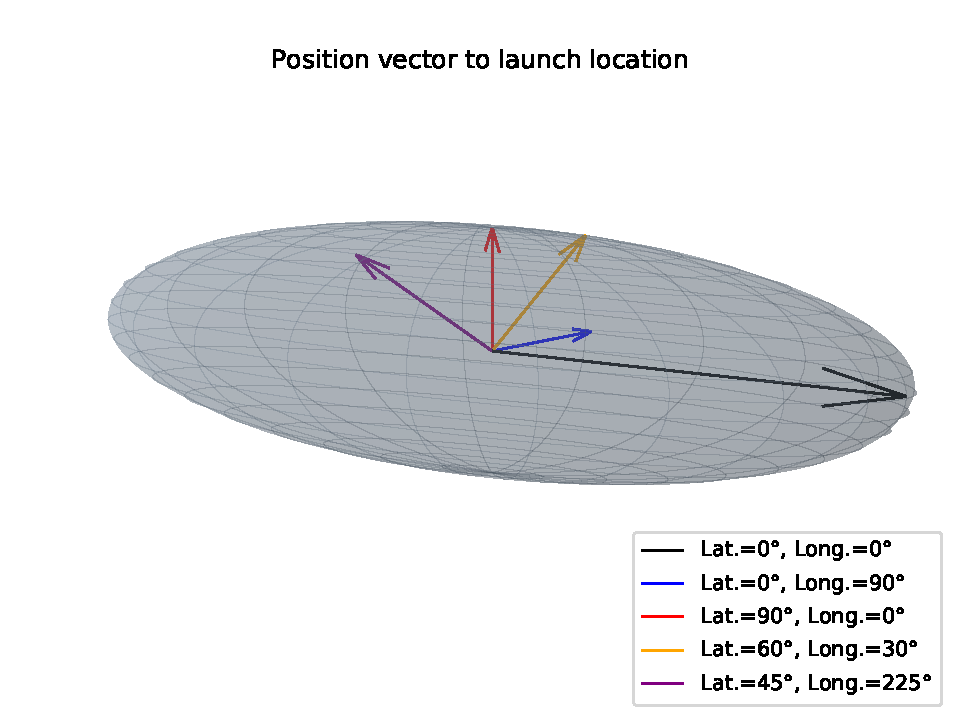
\includegraphics[width=\textwidth, height=0.4\textheight, keepaspectratio=true]{Images/launch_location_position_vectors_2.pdf}
    \label{fig:launch_location_vv_2}
    }
\caption{Position vectors from \protect\Cref{tab:position_vector_to_lat_long_vv} shown with the \protect\gls{CDE} asteroid model.}
\label{fig:position_vector_diagram}
\end{figure}
\FloatBarrier
%%%
We also checked whether the launch location in fact did lie exactly on the surface of the \gls{CDE} asteroid and not inside or above the surface. This is really important because a wrong initial condition could produce erroneous results. Once we substitute the Cartesian coordinates into the triaxial ellipsoid equation (see \Cref{eqn:launch_loc_ellipsoid_eqn_cartesian}) and if the output equals zero (when we take the term 1.0 on the right hand side in \Cref{eqn:launch_loc_ellipsoid_eqn_cartesian}), then the launch point lies on the asteroid. We did an external validation for this but an internal validation always takes place within the dynamics simulator at all times whenever a new simulation is run.
%%%
\begin{table}[htb]
\centering
\captionsetup{justification=centering}
\caption{Output of the triaxial ellipsoid equation for a few test launch location position vectors. An output of 0.0 means that the position vector is a perfect root of the equation and hence the launch location indeed lies on the surface of the asteroid.}
\label{tab:launch_location_surface_vv}
\begin{tabular}{|c|c|c|c|}
\hline
\textbf{X {[}m{]}} & \textbf{Y {[}m{]}} & \textbf{Z {[}m{]}} & \textbf{Output of triaxial ellipsoid equation} \\ \hline
20000.0 & 0.0 & 0.0 & 0.0 \\ \hline
0.0 & 7000.0 & 0.0 & 0.0 \\ \hline
0.0 & 0.0 & 7000.0 & 0.0 \\ \hline
3316.14545023 & 1914.57746836 & 6632.29090046 & 2.22044604925e-16 \\ \hline
-3961.38284482 & -3961.38284482 & 5602.2413449 & 0.0 \\ \hline
\end{tabular}
\end{table}
\FloatBarrier
%%%

\subsection{Launch Velocity}
\label{subsec:launch_velocity_vv}
The launch velocity vector is formed by providing two angles and a magnitude. As explained in \Cref{subsec:launch_velocity}, the two angles are the declination angle from the normal vector at the launch location and the azimuth angle from the local North direction. The local North direction and the normal vector, in essence, act as the basis vectors for a local surface frame of reference which in turn help in the mathematical formulation of the velocity vector of Cartesian components. Since we are dealing with an ellipsoid and not a sphere, defining local North is not a straight-forward process as explained earlier in \Cref{subsec:launch_velocity}.
%
\newline\newline
%
Thus, we first begin with verifying our methodology of forming the local surface frame, and ensure that the local Normal vector and the local North pointing vector are correctly formed and their lies no discrepancy. Then we verify whether the velocity vector, in terms of its Cartesian components, indeed makes the same angle with the surface frame as specified at the input of the simulation. The process for the second verification item is different from how the velocity vector was formed in the first place and hence the verification itself won't be a tampered or faulty process.
%
\newline\newline
%
Let's first begin with a test launch location at the longest edge of the \gls{CDE}. A graphical depiction of the frame is shown in \Cref{fig:surface_frame}. This is the simplest location to perform any simulation or test because the surface normal vector here will be along the same direction as the position vector to the launch point from the centre of the ellipsoid. This also makes the test in itself a trivial task. Note that the surface normal is also the z-axis for the surface frame at the launch point. So for the current test location, if the cross product of the normal and the position vector is a zero vector, then the normal vector is verified. \Cref{tab:longest_edge_surface_frame_vv} shows the result for this. Following this, if the angle between the normal vector and the x-axis basis vector for the surface frame is \SI{90}{\degree}, then the latter is pointing to the local North direction. This is because for the current test location, any vector perpendicular to the surface normal (or effectively to the launch location position vector) will be along the \SI{0}{\degree} meridian line crossing the test location. A simple dot product (again shown in \Cref{tab:longest_edge_surface_frame_vv}) between the x-axis basis vector of the surface frame and the normal vector will tell us if they are perpendicular to each other or not.
%%%
\begin{table}[htb]
\centering
\captionsetup{justification=centering}
\caption{Surface frame verification at the longest edge of the ellipsoid}
\label{tab:longest_edge_surface_frame_vv}
\begin{tabular}{|l|l|l|l|c|}
\hline
\multicolumn{1}{|c|}{\textbf{Unit Vector}} & \multicolumn{3}{c|}{\textbf{Components}} & \textbf{Operations} \\ \hline
\multicolumn{1}{|c|}{} & \multicolumn{1}{c|}{x} & \multicolumn{1}{c|}{y} & \multicolumn{1}{c|}{z} & \multicolumn{1}{l|}{} \\ \hline
Position ($\buv{r}$) & 1.0 & 0.0 & 0.0 & \multirow{2}{*}{$\buv{r} \times \buv{n}$ = {[}0.0, 0.0, 0.0{]}} \\ \cline{1-4}
Normal ($\buv{n}$) & 1.0 & 0.0 & 0.0 &  \\ \hline
X-axis Surface frame / local North direction ($\buv{x}$) & 0.0 & 0.0 & 1.0 & \multicolumn{1}{l|}{$\buv{x} \cdotp \buv{n}$ = 0.0} \\ \hline
\end{tabular}
\end{table}
\FloatBarrier
%%%
Now, we perform a more generalized and non-trivial test for the surface frame but this time we choose a more general launch location. A test site was chosen at \SI{30}{\degree} longitude and \SI{60}{\degree} latitude. It can be viewed in \Cref{fig:surface_frame_leadingEdge_vv}. Note that at this location, the surface normal vector and the launch position vector will not be aligned. We begin with first verifying that the x-axis basis vector for the surface frame at the current launch site is pointing to North. Another way of stating this is that this vector is tangential to the meridian line, which is running all the way up to the poles. If the x-axis basis vector is indeed tangential to the local meridian, then its x-y plane projection will be collinear to that of the position vector to the launch site.
%%%
\begin{table}[htb]
\begin{adjustwidth}{-1in}{-1in}
\centering
\captionsetup{justification=centering}
\caption{Surface frame verification for test launch location at \SI{30}{\degree} Longitude and \SI{60}{\degree} Latitude, i.e., on the leading edge of the asteroid.}
\label{tab:leading_edge_surface_frame_vv}
\begin{tabular}{|l|c|c|c|c|}
\hline
\multicolumn{1}{|c|}{\textbf{Unit Vector}} & \multicolumn{3}{c|}{\textbf{Components}} & \textbf{Operations} \\ \hline
\multicolumn{1}{|c|}{} & x & y & z & \multicolumn{1}{l|}{} \\ \hline
Position ($\buv{r}$) & 0.4330127 & 0.25 & 0.8660254 & \multirow{2}{*}{\begin{tabular}[c]{@{}c@{}}$\buv{x}_x / \buv{r}_x == \buv{x}_y / \buv{r}_y$ \\ = -1.9621431353\end{tabular}} \\ \cline{1-4}
X-axis Surface frame / local North direction ($\buv{x}$) & -0.8496329 & -0.49053578 & 0.1936455 &  \\ \hline
Normal ($\buv{n}$) & 0.05874547 & 0.27687111 & 0.95910967 & \multicolumn{1}{l|}{$\buv{n} \cdotp \buv{x} = 0.0$} \\ \hline
\end{tabular}
\end{adjustwidth}
\end{table}
\FloatBarrier
%%%
%%%
\begin{figure}[htb]
\centering
\captionsetup{justification=centering}
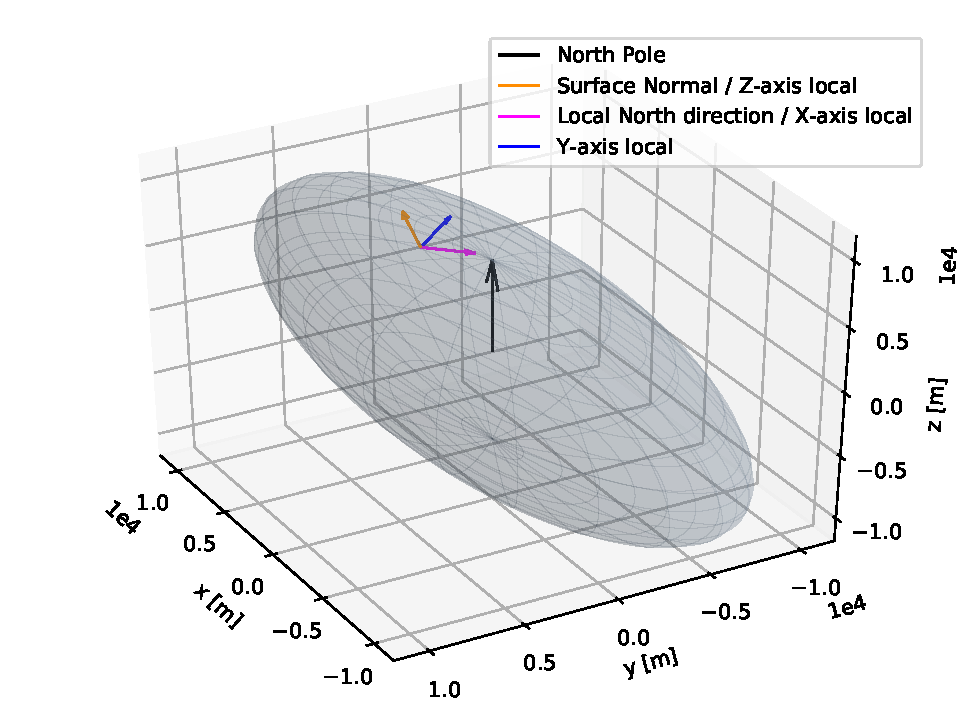
\includegraphics[width=\textwidth, height=0.35\textheight, keepaspectratio=true]{Images/surface_frame_leadingEdge.pdf}
\caption{Surface frame depicted for test launch located at \SI{30}{\degree} Longitude and \SI{60}{\degree} Latitude. Note that the longitude is measured in anti-clockwise direction from the +X axis in the figure.}
\label{fig:surface_frame_leadingEdge_vv}
\end{figure}
\FloatBarrier
%%%
We can prove the two projections to be collinear if the x and the y components of the vectors form equal ratios. This is shown in \Cref{tab:leading_edge_surface_frame_vv}. We see that the ratios are equal and hence the x-axis basis vector is pointing to the North direction. Following this, we can also say that the normal vector at this location is formulated correctly since it is perpendicular to the x-axis basis vector (which in turn is tangential to the meridian line). A vector perpendicular to the meridian line will in-fact be the surface normal vector. Note that, we haven't explicitly verified the y-axis basis vector of the surface frame because it is formed by cross multiplying the normal and the x-axis basis vector. So it inherently remains verified if the latter two are formulated correctly.
%
\newline\newline
%
Now that we have verified that the surface frame is established correctly, we need to verify that the velocity vector makes the correct declination and azimuth angle with the surface frame. The test launch location is still the same as before and the procedure for verification (explained shortly) is different from how the velocity vector was originally formed. We use the vector dot product definition to compute the angle between the velocity vector and the surface normal vector. This gives us the launch declination angle. We then compute the projection of the velocity vector onto the x-y plane of the surface frame \footnote{Given a velocity vector \bvt{v} and the surface normal vector \bvt{n}, the x-y plane projection of \bvt{v} is given as: $\bv{v}_{xy} = \bv{v} - \frac{\bv{v} \cdotp \bv{n}}{n^2} \bv{n}$} and then compute the angle between the projection and the x-axis basis vector of the surface frame. The latter is done, again, by using the dot product method. This then gives us the launch azimuth angle. If the computed angles match the ones provided as input for the simulation, then the velocity vector formulation is verified.
%
\newline\newline
%
Two particle launches were simulated for the aforementioned verification process. The particles were launched with a velocity of 6.0 [m/s] from a point located on the surface of the \gls{CDE} asteroid at \SI{30}{\degree} Longitude and \SI{60}{\degree} Latitude. The first test involved launching particles at declination and azimuth angles of \SI{30}{\degree} and \SI{45}{\degree} respectively. The second test involved declination and azimuth angles of \SI{60}{\degree} and \SI{135}{\degree} respectively. The results for these test simulations is shown in \Cref{tab:launch_velocity_angle_vv_1,tab:launch_velocity_angle_vv_2}. \Cref{fig:launch_velocity_angles_vv} shows the orientation of the velocity vector, for the first test, with respect to the launch site surface frame and the \gls{ARF}.
%%%
\begin{table}[htb]
\begin{adjustwidth}{-1in}{-1in}
\centering
\captionsetup{justification=centering}
\caption{Launch velocity surface frame angles verification data. Input launch declination = \SI{30}{\degree} and azimuth = \SI{45}{\degree}.}
\label{tab:launch_velocity_angle_vv_1}
\begin{tabular}{|l|c|c|c|c|c|}
\hline
\multicolumn{1}{|c|}{\textbf{Vector}} & \multicolumn{3}{c|}{\textbf{\begin{tabular}[c]{@{}c@{}}Vector\\ Components\end{tabular}}} & \textbf{\begin{tabular}[c]{@{}c@{}}Launch\\ Declination {[}deg{]}\end{tabular}} & \textbf{\begin{tabular}[c]{@{}c@{}}Launch\\ Azimuth {[}Deg{]}\end{tabular}} \\ \hline
\multicolumn{1}{|c|}{} & x & y & z &  &  \\ \hline
Velocity ($\bv{v}$) {[}m/s{]} & -0.385325 & -1.354695 & 5.832351 &  & \multicolumn{1}{l|}{\cellcolor[HTML]{9B9B9B}} \\ \cline{1-4}
Unit Normal & 0.058745 & 0.276871 & 0.959109 & \multirow{-2}{*}{30.0} & \multicolumn{1}{l|}{\multirow{-2}{*}{\cellcolor[HTML]{9B9B9B}}} \\ \hline
$\bv{v}$ projection {[}m/s{]} & -0.690575 & -2.793360 & 0.848671 & \multicolumn{1}{l|}{\cellcolor[HTML]{9B9B9B}} &  \\ \cline{1-4}
Unit x-axis surface frame & -0.8496329 & -0.49053578 & 0.1936455 & \multicolumn{1}{l|}{\multirow{-2}{*}{\cellcolor[HTML]{9B9B9B}}} & \multirow{-2}{*}{45.0} \\ \hline
\end{tabular}
\end{adjustwidth}
\end{table}
\FloatBarrier
%%%
%%%
\begin{table}[htb]
\begin{adjustwidth}{-1in}{-1in}
\centering
\captionsetup{justification=centering}
\caption{Launch velocity surface frame angles verification data. Input launch declination = \SI{60}{\degree} and azimuth = \SI{135}{\degree}.}
\label{tab:launch_velocity_angle_vv_2}
\begin{tabular}{|l|c|c|c|c|c|}
\hline
\multicolumn{1}{|c|}{\textbf{Vector}} & \multicolumn{3}{c|}{\textbf{\begin{tabular}[c]{@{}c@{}}Vector\\ Components\end{tabular}}} & \textbf{\begin{tabular}[c]{@{}c@{}}Launch\\ Declination {[}deg{]}\end{tabular}} & \textbf{\begin{tabular}[c]{@{}c@{}}Launch\\ Azimuth {[}Deg{]}\end{tabular}} \\ \hline
\multicolumn{1}{|c|}{} & x & y & z &  &  \\ \hline
Velocity ($\bv{v}$) {[}m/s{]} & 5.223625 & -0.4029416 & 2.924273 &  & \multicolumn{1}{l|}{\cellcolor[HTML]{9B9B9B}} \\ \cline{1-4}
Unit Normal & 0.058745 & 0.276871 & 0.959109 & \multirow{-2}{*}{60.0} & \multicolumn{1}{l|}{\multirow{-2}{*}{\cellcolor[HTML]{9B9B9B}}} \\ \hline
$\bv{v}$ projection {[}m/s{]} & 5.047389 & -1.2335549 & 0.046944 & \multicolumn{1}{l|}{\cellcolor[HTML]{9B9B9B}} &  \\ \cline{1-4}
Unit x-axis surface frame & -0.8496329 & -0.4905357 & 0.1936455 & \multicolumn{1}{l|}{\multirow{-2}{*}{\cellcolor[HTML]{9B9B9B}}} & \multirow{-2}{*}{135.0} \\ \hline
\end{tabular}
\end{adjustwidth}
\end{table}
\FloatBarrier
%%%
%%%
\begin{figure}[htb]
\centering
\captionsetup{justification=centering}
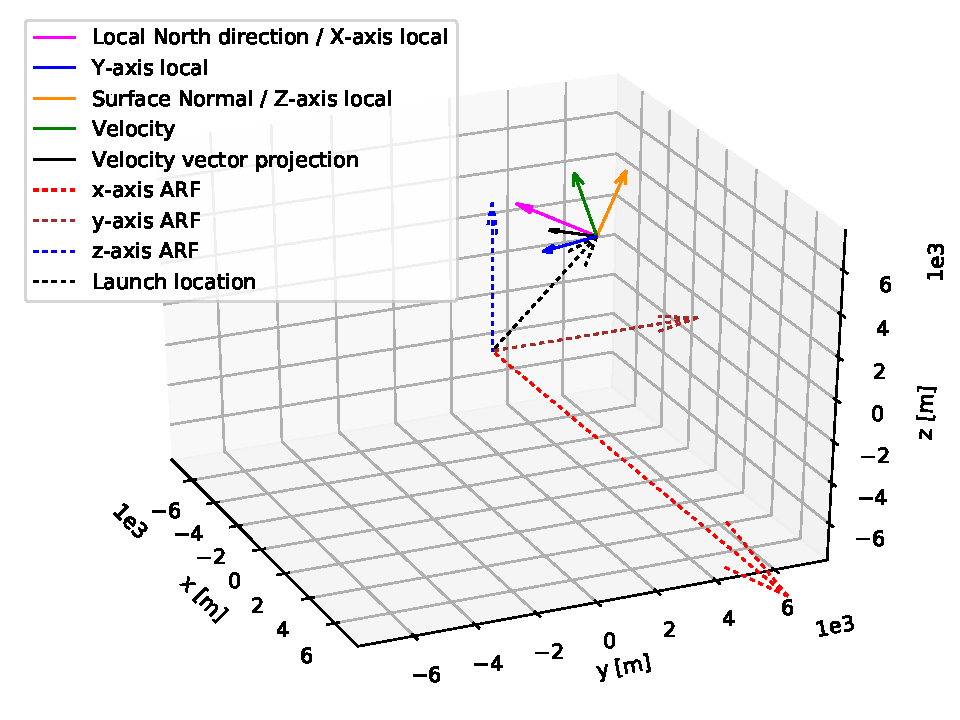
\includegraphics[width=\textwidth, height=0.6\textheight, keepaspectratio=true]{Images/velocity_vector_angles_vv.pdf}
\caption{Schematic representing the surface frame for launch site at \SI{30}{\degree} Longitude and \SI{60}{\degree} Latitude along with the velocity vector and the \gls{ARF}. The diagram gives an intuition on the orientation of the velocity vector. The launch declination and azimuth angles are \SI{30}{\degree} and \SI{45}{\degree} respectively.}
\label{fig:launch_velocity_angles_vv}
\end{figure}
\FloatBarrier
%%%

\section{Regolith Orbital Motion}
\label{sec:orbital_motion_vv}
In this section, we will present results on test simulations that verify and validate the numerical integration of the equations of motion for the regolith in \gls{NAOS}, and in extension, the numerical integrator, the gravity potential model and the relatively smaller functional aspects of the simulator. The tests were done by using the \gls{CDE} gravity potential model, which means that gravity perturbations were accounted for, but excluded the Solar perturbations. This is so that we can test the validity of the simulator by observing the conservation properties of the Jacobi Integral and the Keplerian Energy of an orbiting particle. Both of these would not be conserved if perturbations were included in the test.

\subsection{Spherical Asteroid}
\label{subsec:spherical_asteroid__orbital_mech_vv}
We first test the simulator for a particle launched from the surface of a spherical asteroid of radius \SI{20}{\kilo \metre}. The launch site was located at \SI{0}{\degree} Longitude and Latitude. A single particle was launched with a velocity of \SI{10.0}{\metre \per \second} with an azimuth angle of \SI{135}{\degree} and declination angle of \SI{45}{\degree}. Note that the \gls{CDE} potential model was still used for this simulation with all three semi-major axes made equal to the sphere radii. If the gravity potential model is formulated properly, then with all three semi-major axes being equal, the potential model will act like a point-mass model. This would make the gravity field uniform and hence conserve the Keplerian Energy. The Jacobi integral and the Keplerian energy for this test is shown in \Cref{fig:spherical_asteroid_jacobi_energy_vv}. From the conservation of these values, we can infer that atleast for a spherical asteroid, the simulator works correctly.
%%%
\begin{figure}[htb]
\centering
\captionsetup{justification=centering}
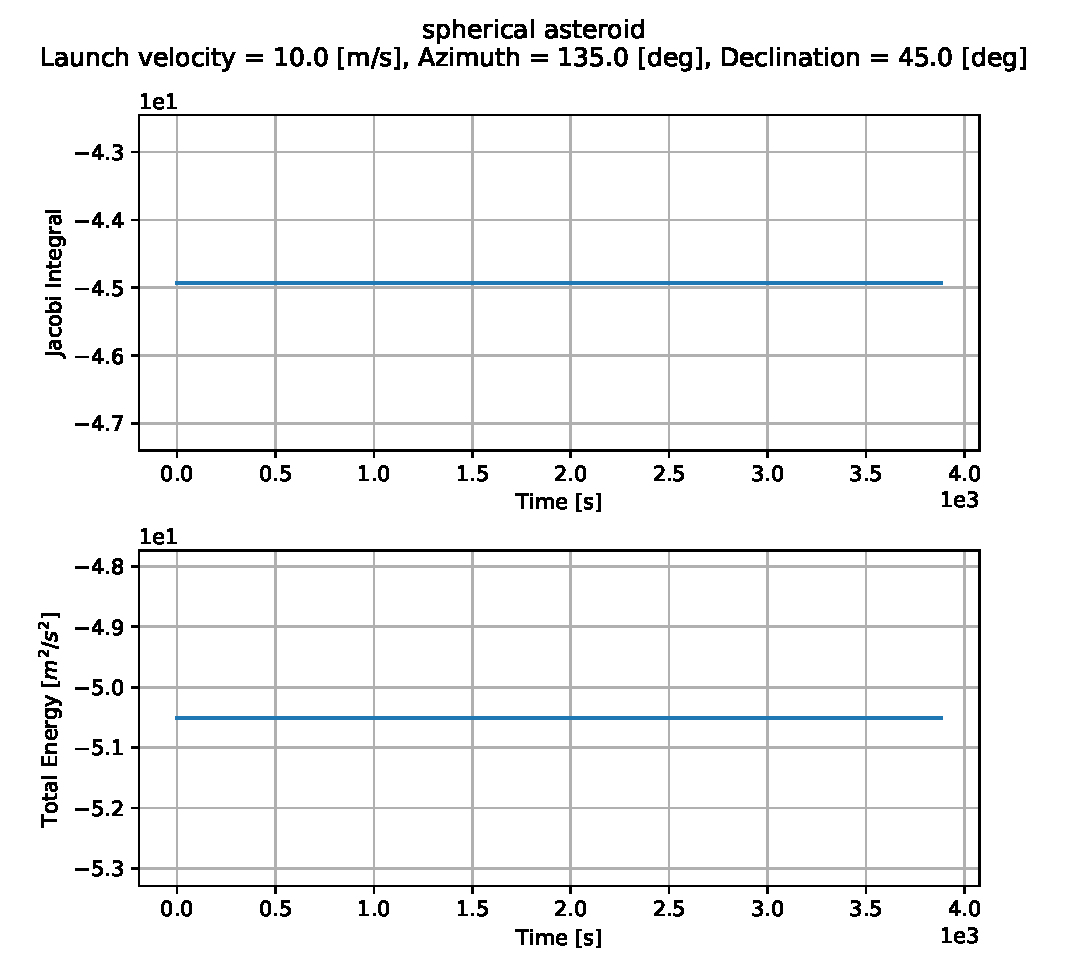
\includegraphics[width=\textwidth, height=0.5\textheight, keepaspectratio=true]{Images/spherical_asteroid_jacobi_energy.pdf}
\caption{Jacobi Integral and Keplerian Energy for the regolith launched from the surface of a spherical asteroid at Latitude and Longitude \SI{0}{\degree} remains conserved.}
\label{fig:spherical_asteroid_jacobi_energy_vv}
\end{figure}
\FloatBarrier
%%%

\subsection{\gls{CDE} Asteroid}
\label{subsec:CDE_asteroid_orbital_mech_vv}
We'll perform a similar test as before but this time for a \gls{CDE} shaped asteroid of semi-major axes $\alpha$ = \SI{20}{\kilo \metre}, $\beta$ = \SI{7}{\kilo \metre}, $\gamma$ = \SI{7}{\kilo \metre}. A single regolith was launched from the surface at site Longitude \SI{30}{\degree} and Latitude \SI{60}{\degree}. The particle was launched with a velocity of \SI{10}{\metre \per \second}, azimuth angle of \SI{135}{\degree} and declination angle of \SI{30}{\degree}. Now since the gravity potential model is a non-uniform one, unlike that in the case of the spherical asteroid, the Jacobi integral would remain conserved however the Keplerian energy of the particle should not remain conserved. We see this outcome in \Cref{fig:cde_asteroid_jacobi_energy_vv}. This result further validates the simulator since the Jacobi remains conserved, implying that the equations of motion, the gravity potential model, the numerical integrator and several other background functions of the simulator work correctly.
%%%
\begin{figure}[htb]
\centering
\captionsetup{justification=centering}
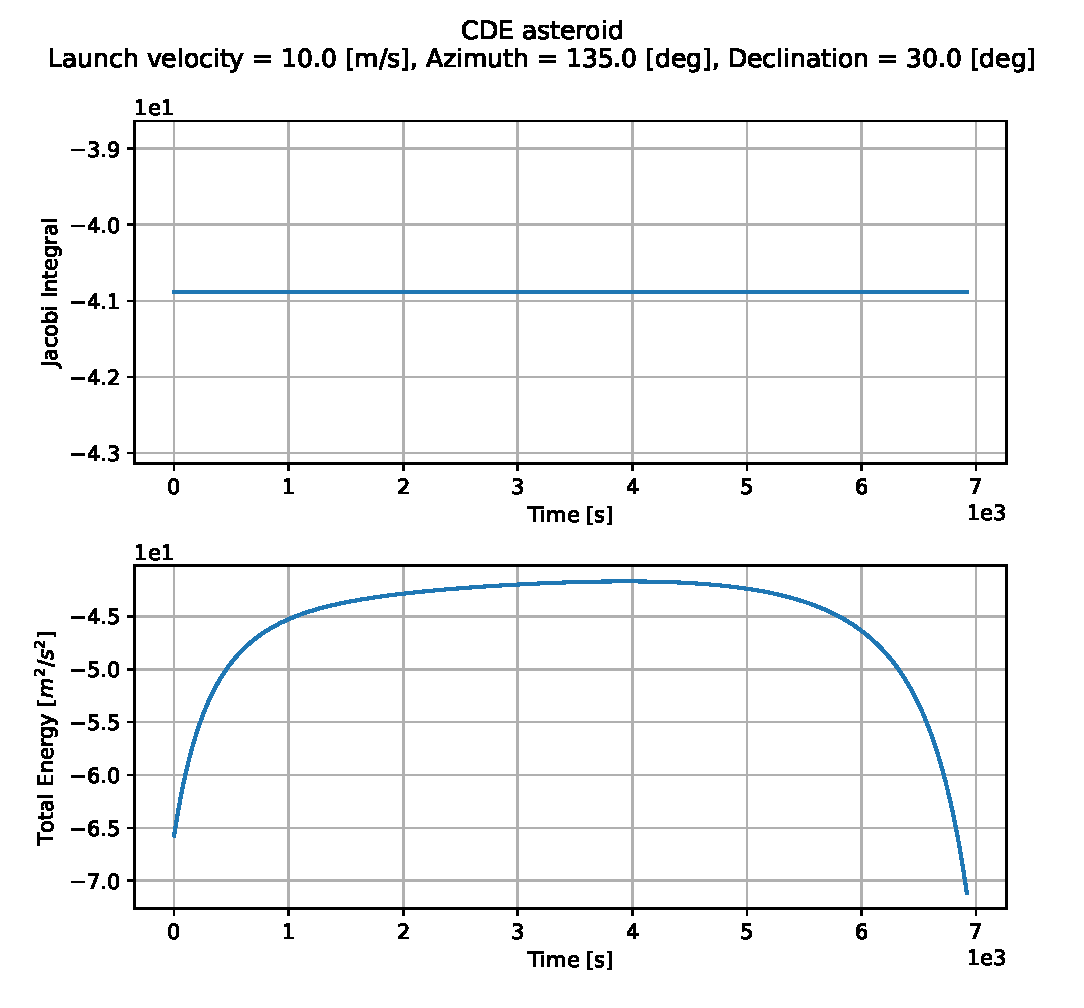
\includegraphics[width=\textwidth, height=0.5\textheight, keepaspectratio=true]{Images/cde_asteroid_long30_lat60_jacobi_energy.pdf}
\caption{Jacobi Integral and Keplerian Energy for the regolith launched from the surface of a \gls{CDE} shaped asteroid at Latitude \SI{60}{\degree} and Longitude \SI{30}{\degree}.}
\label{fig:cde_asteroid_jacobi_energy_vv}
\end{figure}
\FloatBarrier
%%%
Post this, two other tests were performed from the leading edge of the asteroid, one of which resulted in re-impact and the other which resulted in an escape situation. The Jacobi integral for the two simulation was computed which again turned out to be constant throughout the duration of the respective trajectories. The results and initial conditions for the re-impact case are shown in \Cref{fig:cde_asteroid_jacobi_reimpact_vv} and for the escape case are shown in \Cref{fig:cde_asteroid_jacobi_escape_vv}. The launch declination in both cases is \SI{45}{\degree}. The results further validate the functionality of the simulator.
%%%
\begin{figure}[htb]
% \begin{adjustwidth}{-1in}{-1in}
\centering
\captionsetup{justification=centering}
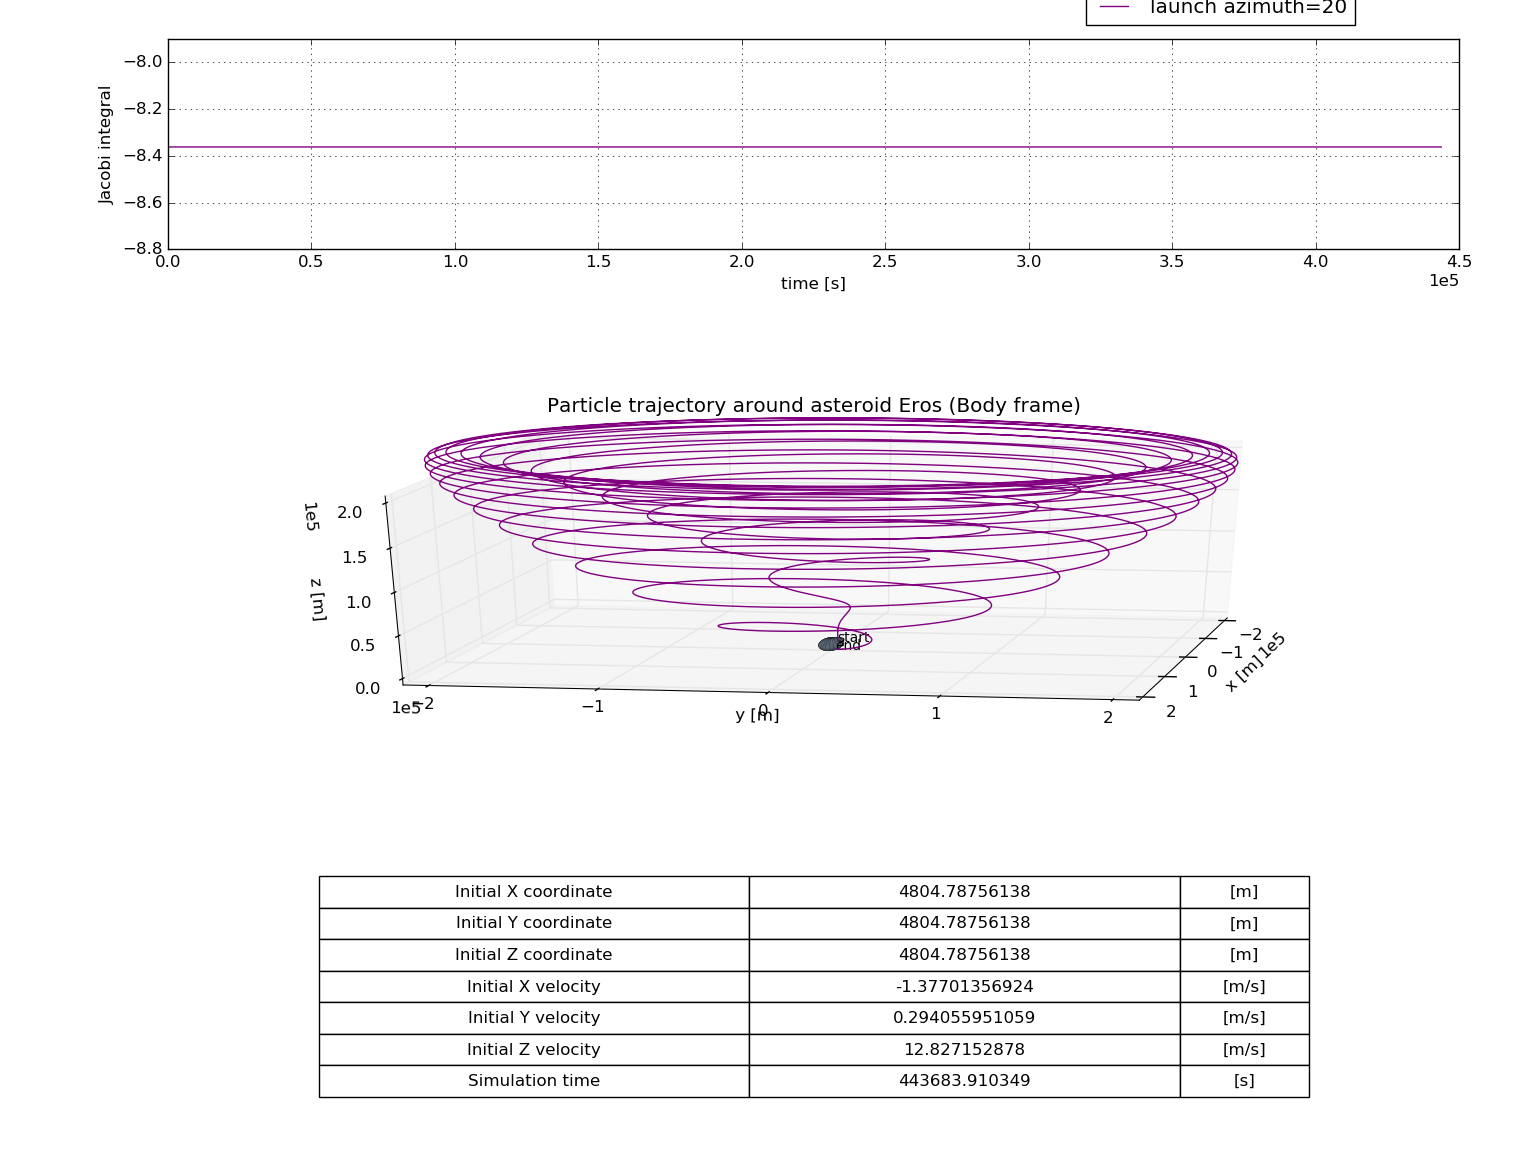
\includegraphics[angle=90, height=0.8\textheight, keepaspectratio=true]{Images/jacobi_test_after_asteroid_interaction_long_term_simulation.png}
\caption{Jacobi Integral for the regolith launched from the leading edge of a \gls{CDE} shaped asteroid which eventually re-impacts the surface of the asteroid.}
\label{fig:cde_asteroid_jacobi_reimpact_vv}
% \end{adjustwidth}
\end{figure}
\FloatBarrier
%%%
%%%
\begin{figure}[htb]
\centering
\captionsetup{justification=centering}
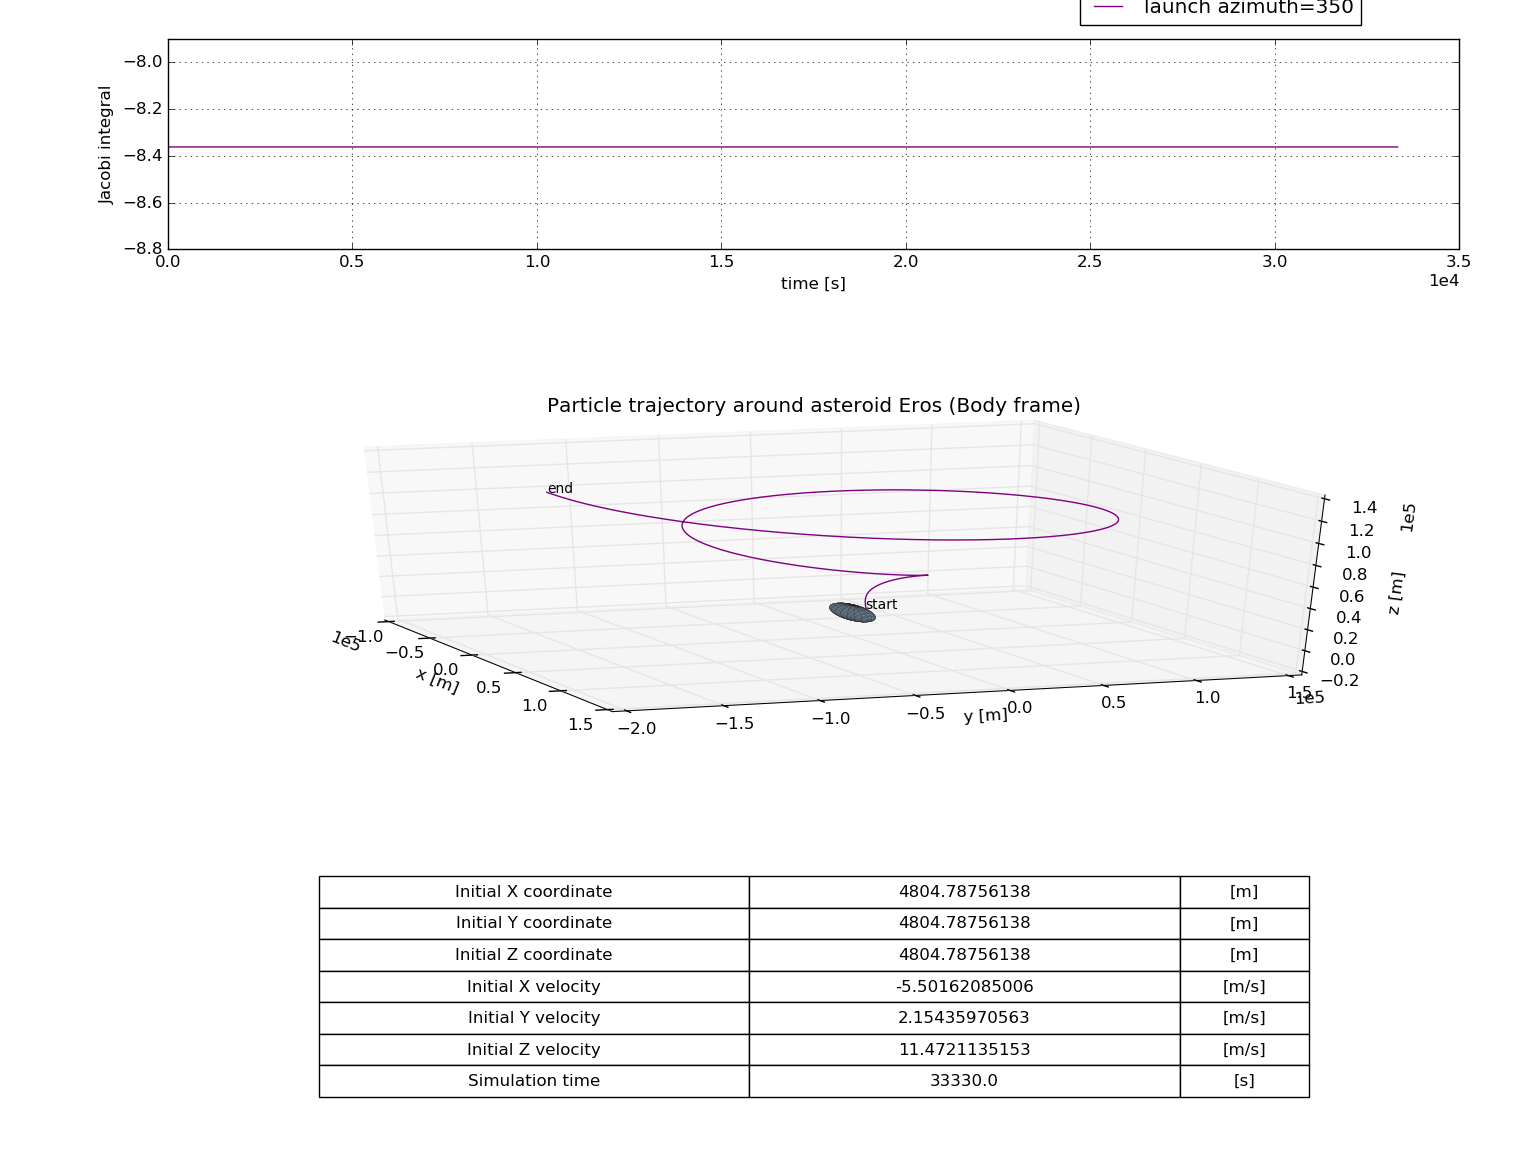
\includegraphics[width=\textwidth, height=0.6\textheight]{Images/jacobi_test_for_escaped_particle.png}
\caption{Jacobi Integral for the regolith launched from the leading edge of a \gls{CDE} shaped asteroid which eventually escapes the gravitational attraction of the asteroid.}
\label{fig:cde_asteroid_jacobi_escape_vv}
\end{figure}
\FloatBarrier
%%%

\subsection{Integrator Performance}
\label{subsec:integrator_tuning_vv}
The integrator used in our simulator \gls{NAOS} was from an external library called \emph{boost}. We use this library because coding higher order numerical integrators is an extremely daunting task which would have swayed away time and focus from the thesis at hand. On top of that, the boost library provides verified integrator subroutines (among other things) and hence this reduces our task to just verify that it has been used properly in our simulator. From the results in the previous two subsections, we can say that the integrator has been properly accommodated in \gls{NAOS} otherwise the behavior of the Jacobi integral and the Keplerian energy would have been different. Here, we will briefly discuss the performance of the integrator under different configurations of itself, for the same particle launch conditions as mentioned in \Cref{subsec:CDE_asteroid_orbital_mech_vv}. But first we'll give a brief description of the integrators adaptive behavior before we can look at some numbers on the performance.
%
\newline\newline
%
The integrator used is a Runge-Kutta-Fehlberg78, which is an 8th order integrator with the 7th order used for error control. The integrator uses an adaptive step size, which means that the step size for integration, from one epoch to another, changes continuously depending on the magnitude of integration error at each step. What this means is that the number of steps taken to integrate from an initial epoch to the final one changes, for every instance of integration in a sequence. So to propagate the state vector from, say, time $t_0$ to $t_1$, the integrator first performs a single step of integration based on an initial guess for the step-size. This is done first using an order 8 process then again using a 7th order process. The difference in the outcome between the two is then treated as the numerical error for that step. This process of error estimation of-course repeats for every other step of integration performed, to go from time $t_0$ to $t_1$. The estimated error is compared with the following equation:
\begin{align}
abs_{tol} + rel_{tol} \times ( X + ( dt * dXdt ) )
\label{eqn:integrator_abs_rel_tol}
\end{align}
where $abs_{tol}$ and $rel_{tol}$ are the absolute and relative error tolerances of the integrator, and their values can be set by the user; $X$ is the state vector, $dt$ is the time step for integration, and $dXdt$ is the first order differential equation for the state vector (so basically the equations of motion in our case). Now if the estimated error is smaller than \Cref{eqn:integrator_abs_rel_tol}, the integration step is accepted and the integrator moves on to the next step. If, however, the estimated error is larger, then the step size is reduced and the integration is performed again. There are other processes that run internally
within the subroutine, that ensure that the step-size does not become too small or too large, the details of which can be found at \parencite{boost_odeint}.
%
\newline\newline
%
\Cref{tab:integrator_performance} gives values for certain metrics that showcase the variation in performance of the Runge-Kutta-Fehlberg78 integrator. Note that we propagated the trajectory of the regolith for the same initial conditions as mentioned in \Cref{subsec:CDE_asteroid_orbital_mech_vv}. The metric CPU time refers to the total time taken by the computer processor to integrate the entire problem from start to end. The total CPU time shouldn't be taken at face value but rather at the order of magnitude because background processes in the computer could delay the time taken to perform a given simulation. The entire simulation, from the start till the end, is broken down into a series of smaller integration instances. For each instance then, the number of steps to perform the integration changes since the step-size keeps on changing. Thus, the column \emph{max. step} refers to the maximum number of steps undertaken for any integration instance in the entirety of the simulation. Similarly, the column \emph{min. step} gives the values for the least number of steps. Each row in \Cref{tab:integrator_performance} corresponds to one entire simulation performed with the given absolute and relative tolerances.
%%%
\begin{table}[htb]
\centering
\captionsetup{justification=centering}
\caption{Variation in integrator performance for different error tolerance values.}
\label{tab:integrator_performance}
\begin{tabular}{|c|c|c|c|c|}
\hline
\textbf{\begin{tabular}[c]{@{}c@{}}Absolute\\ Tolerance\end{tabular}} & \textbf{\begin{tabular}[c]{@{}c@{}}Relative\\ Tolerance\end{tabular}} & \textbf{CPU time {[}s{]}} & \textbf{Max. Steps} & \textbf{Min. Steps} \\ \hline
$10^{-2}$ & $10^{-2}$ & 0.54 & 6 & 3 \\ \hline
$10^{-6}$ & $10^{-6}$ & 0.47 & 6 & 3 \\ \hline
$10^{-15}$ & $10^{-15}$ & 0.41 & 6 & 3 \\ \hline
$10^{-20}$ & $10^{-20}$ & 2.43 & 2468 & 5 \\ \hline
\end{tabular}
\end{table}
\FloatBarrier
%%%
It is important to note that the integrity of the simulation from the dynamics point of view was not hampered for any of the combinations of absolute and relative tolerances given in \Cref{tab:integrator_performance}. They all gave the same result as that in \Cref{fig:cde_asteroid_jacobi_energy_vv}. A logical inference to be drawn from this is that even when the tolerance is relatively large, the simulation results turn out to be the same because the estimated error in integration itself is very small in the first place. We see a visible difference in the performance only when the tolerances are made extremely small, such as $10^{-20}$, which ultimately causes the integrator to perform computations at much smaller step-sizes because now the estimated error gets larger in comparison to \Cref{eqn:integrator_abs_rel_tol}. Not shown in \Cref{tab:integrator_performance}, but the tolerances were further reduced to $10^{-30}$ at which point the simulation got extremely slow and never ceased within a reasonable amount of time. Thus extremely small tolerances, i.e. beyond $10^{-15}$, should not used for the purposes of this thesis since we are simulating several thousand particles at the same time. We ultimately decided to use an absolute and relative tolerance of $10^{-15}$ since it gave the same performance as any other higher tolerance value.

\section{Solar Perturbations}
\label{sec:perturbations_vv}
In this section we will provide results on tests performed to validate the perturbing force models. The test data was taken from, the already verified, unit test files of \gls{TUDAT} \footnote{\gls{TUDAT} is an open source astrodynamics toolbox, developed and maintained by the department of astrodynamics and space missions at the Delft University of Technology and the toolbox can be found at \url{https://github.com/tudat/}.}. We benchmark the force models used in \gls{NAOS} by performing tests with data from \gls{TUDAT} and data obtained from some simplified hand-based calculations as well. The subroutines for the force models in \gls{NAOS} were modular enough and no changes were made to the function codes to accommodate the validation process.

\subsection{Solar Third-Body Effect}
\label{subsec:stbe_vv}
We'll begin by presenting validation data for the \gls{STBE} perturbing acceleration. The position vector of the target location where the perturbing acceleration had to be calculated, and the position vector to a random perturbing body, are both mentioned with respect to some common arbitrary frame of reference. The definition of the latter does not matter or affect the computation within the \gls{STBE} force model. The gravitational parameter of the perturbing body is \SI{4900.0e9}{\metre \cubed \per \second \squared}. The computed acceleration values matched those provided in the \gls{TUDAT} unit test files, shown in \Cref{tab:stbe_vv_tudat_data}, thus validating the \gls{STBE} force model for a more generalized 3D data.
%%%
\begin{table}[htb]
\centering
\captionsetup{justification=centering}
\caption{Validation data for testing the \gls{STBE} force model, taken from unit test files in \gls{TUDAT}. The gravitational parameter of the perturbing body is \SI{4900.0e9}{\metre \cubed \per \second \squared}.}
\label{tab:stbe_vv_tudat_data}
\begin{tabular}{|l|c|c|c|}
\hline
\multicolumn{1}{|c|}{\textbf{Vector}} & \multicolumn{3}{c|}{\textbf{Component}} \\ \hline
\multicolumn{1}{|c|}{} & x & y & z \\ \hline
Target position {[}m{]} & -40000000.0 & 9000000.0 & -9500000.0 \\ \hline
Perturber position {[}m{]} & 25000000.0 & -380000000.0 & -55000000.0 \\ \hline
Perturbing acceleration {[}\si{\metre \per \second \squared}{]} & 2.93946e-06 & 2.22539e-06 & 1.16801e-06 \\ \hline
\end{tabular}
\end{table}
\FloatBarrier
%%%
The second test was a more simplified one and uses hand-based calculations to verify the software routine. This was done to test if the routine performs correctly even for an edge case. The test considers a planar situation wherein the regolith is on the positive x-axis with respect to the asteroid (consider looking at \Cref{fig:stbe_inertialFrame} to visualize the set up) and the Sun is in the equatorial plane of the asteroid on the negative x-axis. The position vectors for the two bodies and the corresponding acceleration values, both hand-calculated and software computed, are shown in \Cref{tab:stbe_vv_handcalculated_data}.
%%%
\begin{table}[htb]
\centering
\captionsetup{justification=centering}
\caption{Validating the \gls{STBE} force model using hand-calculated acceleration values for a specific edge case.}
\label{tab:stbe_vv_handcalculated_data}
\begin{tabular}{|l|c|c|c|c|}
\hline
\multicolumn{2}{|c|}{\textbf{Vector}} & \multicolumn{3}{c|}{\textbf{Component}} \\ \hline
\multicolumn{2}{|c|}{} & x & y & z \\ \hline
\multicolumn{2}{|l|}{Target position {[}m{]}} & 25000.0 & 0.0 & 0.0 \\ \hline
\multicolumn{2}{|l|}{Perturber position {[}m{]}} & -1.0 AU & 0.0 & 0.0 \\ \hline
\multirow{2}{*}{Perturbing acceleration {[}\si{\metre \per \second \squared}{]}} & Hand-calculated & 1.98201e-09 & 0.0 & 0.0 \\ \cline{2-5}
 & Software computed & \multicolumn{1}{l|}{1.98201e-09} & \multicolumn{1}{l|}{-3.64089e-25} & \multicolumn{1}{l|}{0.0} \\ \hline
\end{tabular}
\end{table}
\FloatBarrier
%%%
There is an extremely small round off error in the y-component of the software computed perturbation acceleration but apart from that the software values match the hand-calculated ones in terms of both magnitude and direction.

\subsection{Solar Radiation Pressure}
\label{subsec:srp_vv}
We'll now present validation data for the \gls{SRP} force model. The first test assumes a spacecraft near Venus. The parametric data for the test was again taken from the \gls{TUDAT} unit test files and is shown in \Cref{tab:srp_vv_tudat_data_1}. The acceleration due to \gls{SRP} computed from the software routine matched in direction and magnitude with the test data. The position vector goes from the target to the Sun and is defined with respect to an arbitrary frame. The definition of the frame does not matter for the software routine to calculate the perturbing accelerations, apart from the fact that the values will be defined with respect to the arbitrary frame.
%%%
\begin{table}[htb]
\centering
\captionsetup{justification=centering}
\caption{Validation of \gls{SRP} model using test data from \gls{TUDAT}. The test assumes a satellite somewhere near Venus and considers a planar case.}
\label{tab:srp_vv_tudat_data_1}
\begin{tabular}{|l|l|}
\hline
\multicolumn{1}{|c|}{\textbf{Parameter}} & \multicolumn{1}{c|}{\textbf{Value}} \\ \hline
Target to Sun position vector {[}m{]} (x, y, z) & (77432181578.46405, 77432181578.46405, 0.0) \\ \hline
Target emissivity & 0.5 \\ \hline
Solar incident area {[}\si{\metre \squared}{]} & 0.005 \\ \hline
Target mass {[}kg{]} & 0.0022 \\ \hline
Solar constant & 1.0205062450596109e+17 \\ \hline
Perturbing acceleration {[}\si{\metre \per \second \squared}{]} (x, y, z) & (-2.05148e-05, -2.05148e-05, 0.0) \\ \hline
\end{tabular}
\end{table}
\FloatBarrier
%%%
The second test, again taken from \gls{TUDAT}, assumes a random location for the target in 3D, thus providing a more generalized test scenario. The incident area and target mass are also extremely exaggerated. The parametric data used for the test and the output acceleration values are shown in \Cref{tab:srp_vv_tudat_data_2}.
%%%
\begin{table}[htb]
\centering
\captionsetup{justification=centering}
\caption{Validation of \gls{SRP} model using test data from \gls{TUDAT}. The test assumes an exaggerated target body at a random location and considers a general 3D scenario.}
\label{tab:srp_vv_tudat_data_2}
\begin{tabular}{|l|l|}
\hline
\multicolumn{1}{|c|}{\textbf{Parameter}} & \multicolumn{1}{c|}{\textbf{Value}} \\ \hline
Target to Sun position vector {[}m{]} (x, y, z) & (94359740.25, 90831886.1, 14668782.92) \\ \hline
Target emissivity & 0.4058 \\ \hline
Solar incident area {[}\si{\metre \squared}{]} & 514701.9505 \\ \hline
Target mass {[}kg{]} & 1.0 \\ \hline
Solar constant & 1.0205062450596109e+17 \\ \hline
Perturbing acceleration {[}\si{\metre \per \second \squared}{]} (x, y, z) & (-3.04373e+06, -2.92993e+06, -473166) \\ \hline
\end{tabular}
\end{table}
\FloatBarrier
%%%
The perturbing accelerations computed from the software routine for \gls{SRP} in \gls{NAOS} matches the test data from \gls{TUDAT}, thus validating the software model. Just like for \gls{STBE}, we present a case of validation against hand-calculated data for a set of very simple parametric values. The results and test data are given in \Cref{tab:srp_vv_hand_calc_data}. There is an extremely small round-off error in the x-component of the computed acceleration, but the magnitude and direction matches that of the hand-computed values. Thus with this final test, we can say that the software is verified.
%%%
\begin{table}[htb]
\centering
\captionsetup{justification=centering}
\caption{Validation of \gls{SRP} model in \gls{NAOS} for an edge case against hand-calculated data.}
\label{tab:srp_vv_hand_calc_data}
\begin{tabular}{|l|l|l|}
\hline
\multicolumn{2}{|c|}{\textbf{Parameter}} & \multicolumn{1}{c|}{\textbf{Value}} \\ \hline
\multicolumn{2}{|l|}{Target to Sun position vector {[}m{]} (x, y, z)} & (0.0, 0.1 AU, 0.0) \\ \hline
\multicolumn{2}{|l|}{Target emissivity} & 1.0 \\ \hline
\multicolumn{2}{|l|}{Solar incident area {[}\si{\metre \squared}{]}} & 1.0 \\ \hline
\multicolumn{2}{|l|}{Target mass {[}kg{]}} & 1.0 \\ \hline
\multicolumn{2}{|l|}{Solar constant} & 1.0e+17 \\ \hline
\multicolumn{1}{|c|}{\multirow{2}{*}{Perturbing acceleration {[}\si{\metre \per \second \squared}{]} (x, y, z)}} & Hand-calculated & (0.0, -0.000893674, 0.0) \\ \cline{2-3}
\multicolumn{1}{|c|}{} & Software computed & (-5.47218e-19,-0.000893674, 0.0) \\ \hline
\end{tabular}
\end{table}
\FloatBarrier
%%%

\section{Regolith Final Fate}
\label{sec:final_fate_vv}
Now that we have verified the gravity model, the orbital dynamics and the perturbing force models, the last major validation that we need to perform is to check whether the final fate of a regolith is correctly determined. We do the check for test simulations run from the leading edge of the asteroid while including perturbations. The launch location was at Longitude \SI{30}{\degree} and Latitude \SI{60}{\degree}. Multiple regolith were launched from the site with all possible combinations of the following launch conditions: velocities ranging from \SI{10}{\metre \per \second} to \SI{13}{\metre \per \second}, launch azimuth angles varying in steps of \SI{45}{\degree}, and launch declination angles of \SI{30}{\degree} and \SI{60}{\degree}. The initial Solar phase angle was \SI{315}{\degree}.
%
\newline\newline
%
This set of launch site and initial conditions provides a very generalized scenario for testing the eventual outcome of the regolith. \Cref{fig:finalfate_vv_escape} shows the results for all recorded escape cases from the test simulation. Every particle that has escaped satisfies the necessary condition of having eccentricity greater than or equal to one and energy being positive. Note that these values are given for the final epoch in the simulation i.e. when any of the possible final fates is realized and the simulation is stopped.
%
\newline\newline
%
We can validate the re-impact situations by evaluating the triaxial ellipsoid equation for the state vector at the final epoch of the simulation. This was done for all cases that had been identified, by the simulator, to have re-impacted the surface of the asteroid. If the solution turns out to be zero, then we know that the particle is on the ellipsoid itself. In \Cref{fig:finalfate_vv_crash}, we do see that all impacted particles provide the desired solution to the triaxial ellipsoid equation. The results are shown only for a subset of re-impact cases, i.e., only for those regoliths whose initial velocity was \SI{13}{\metre \per \second}.
%%%
\begin{figure}[htb]
\centering
\captionsetup{justification=centering}
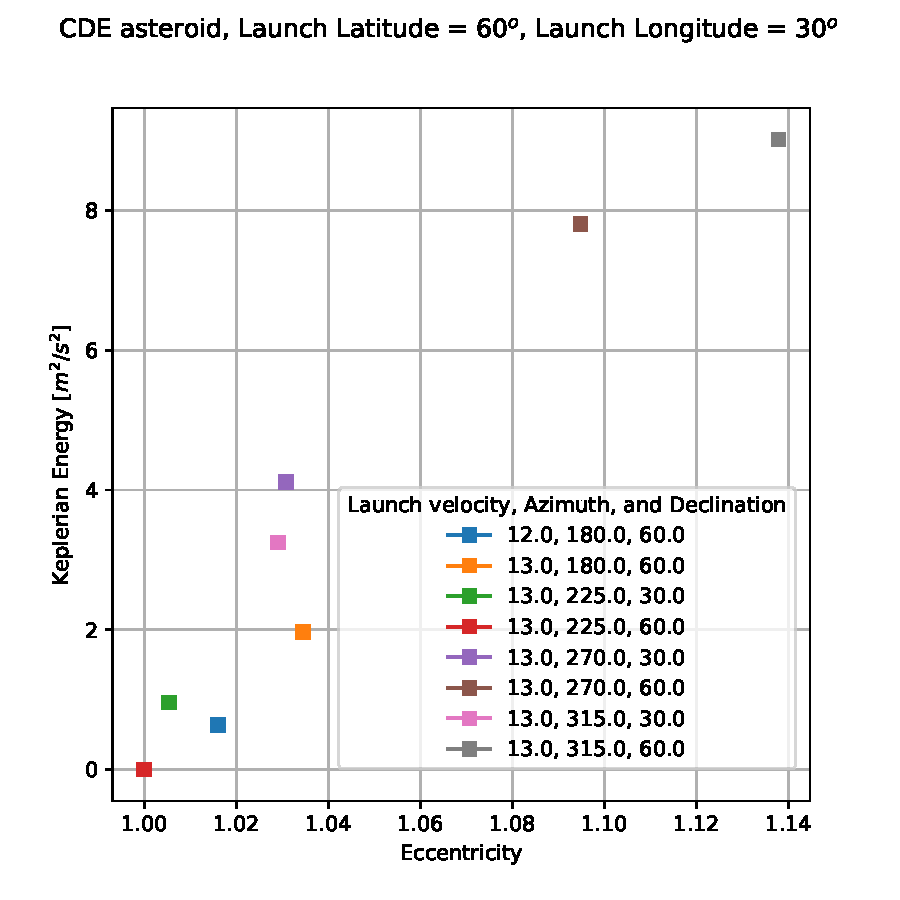
\includegraphics[width=\textwidth, height=0.4\textheight, keepaspectratio=true]{Images/escape_vv.pdf}
\caption{Energy v/s eccentricity plot for regolith that eventually escaped after being launched from the surface of the asteroid. When the energy is positive and eccentricity is greater than or equal to one, the regolith escapes. In the legend, the launch velocity and the two angles are expressed in \si{\metre \per \second} and degrees respectively.}
\label{fig:finalfate_vv_escape}
\end{figure}
\FloatBarrier
%%%
%%%
\begin{figure}[htb]
\centering
\captionsetup{justification=centering}
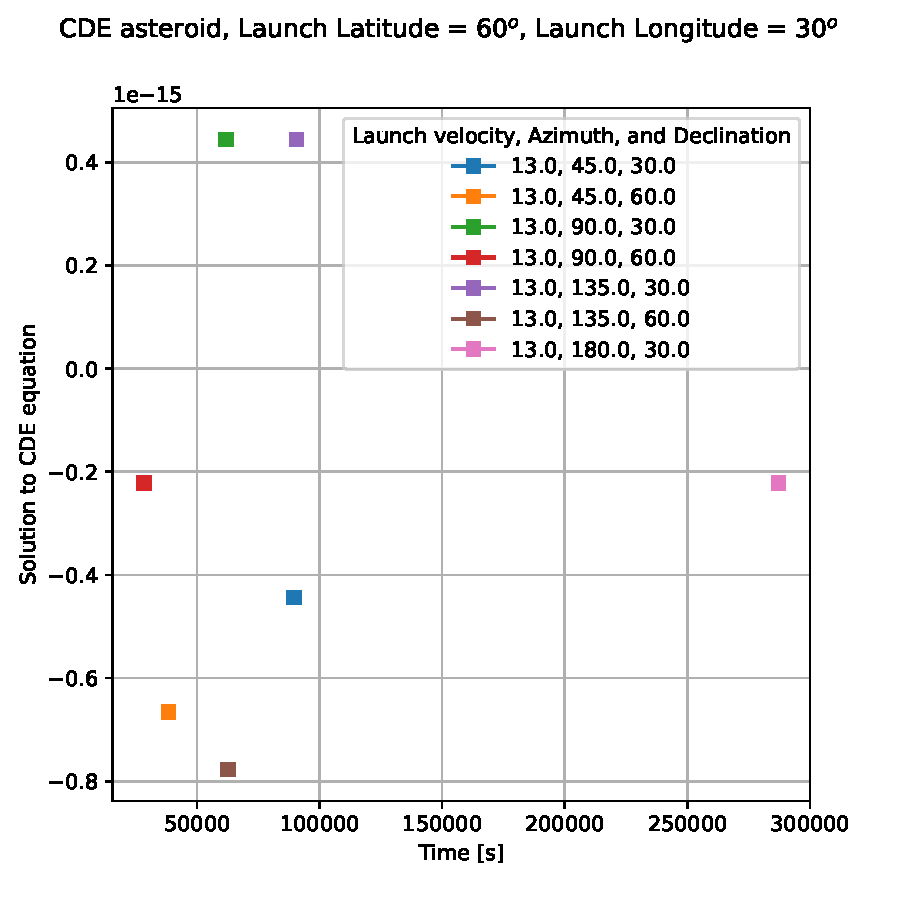
\includegraphics[width=\textwidth, height=0.4\textheight, keepaspectratio=true]{Images/crash_vv.pdf}
\caption{Solution to the triaxial ellipsoid equation for a subset of re-impacted particles. This solution is obtained for the state vector at the final epoch of the simulation, for the given subset of re-impacted particles. In the legend, the launch velocity and the two angles are expressed in \si{\metre \per \second} and degrees respectively.}
\label{fig:finalfate_vv_crash}
\end{figure}
\FloatBarrier
%%%
In the test just performed, from the leading edge of the asteroid, we did not obtain any capture cases. To validate this special final fate, we ran another simulation from the longest edge of the asteroid. Note that a capture case is indirectly detected when the simulator propagates the regolith and it doesn't escape or re-impacts the surface of the asteroid. So we perform an internal passive test for a known capture case, wherein we check that the particle doesn't have escape characteristics when far away from the asteroid and neither does it have re-impact characteristics when extremely close to the asteroid.
%
\newline\newline
%
A single regolith was launched from Longitude and Latitude \SI{0}{\degree}, with launch velocity magnitude of \SI{10}{\metre \per \second}, azimuth angle of \SI{45}{\degree} and declination angle of \SI{45}{\degree}. The initial Solar phase angle was \SI{315}{\degree}. \Cref{fig:capture_vv_energy_eccentricity} shows the osculating Keplerian energy and eccentricity of the regolith when it is far away from the asteroid, i.e., when the range to the particle is equal to or beyond 10 times the largest semi-major axis of the asteroid, which is \SI{200}{\kilo \metre} in this particular case. When far away, the regolith always maintains a negative total Keplerian energy and an eccentricity less than 1.0, thereby staying bounded to the asteroid.
%%%
\begin{figure}[htb]
\centering
\captionsetup{justification=centering}
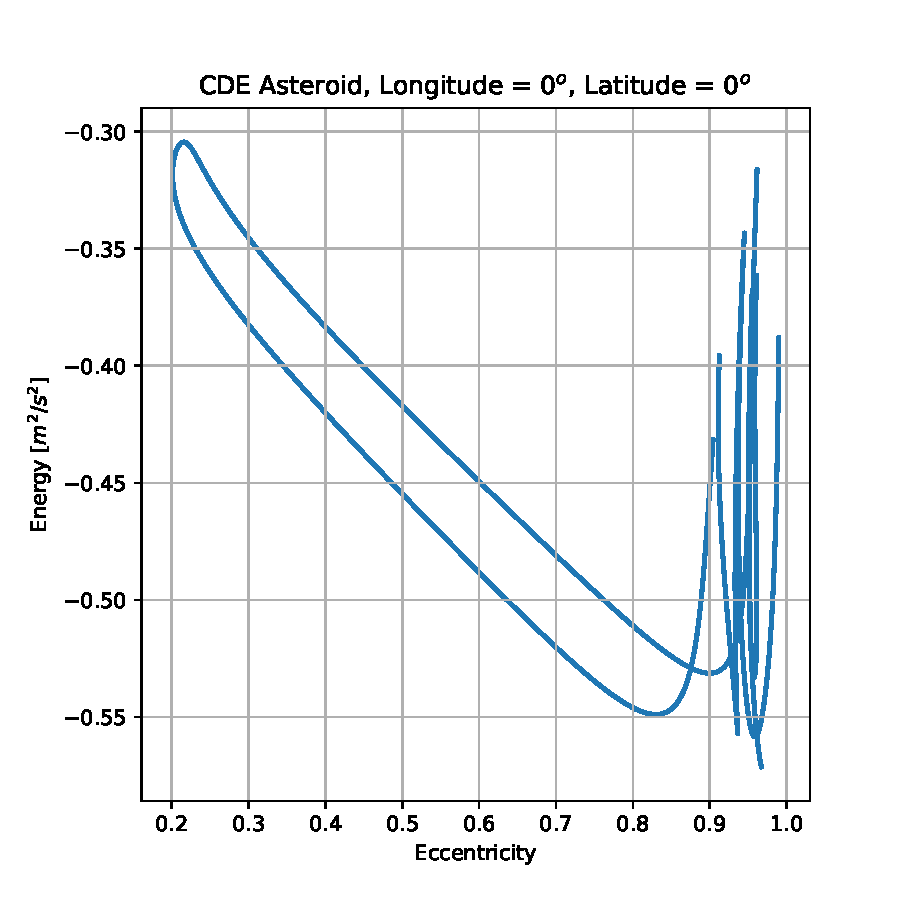
\includegraphics[width=\textwidth, height=0.4\textheight, keepaspectratio=true]{Images/capture_vv_energy_eccentricity_10AlphaUpwards.pdf}
\caption{Osculating Keplerian energy versus eccentricity plot for the regolith with temporary capture as its final fate. The data points plotted here are for the case when the particle has a range beyond 10 times the largest semi-major axis of the \gls{CDE} (i.e. \SI{200}{\kilo \metre} in this test). This check was performed to ensure that the particle does not have escape characteristics when far away from the asteroid.}
\label{fig:capture_vv_energy_eccentricity}
\end{figure}
\FloatBarrier
%%%
The second indirect test is to check if the particle ever interacts with the surface of the asteroid, that goes unnoticed by the simulator for any reason at all. In this regard this test case is special since we witness that the regolith comes extremely close to the asteroid. We do this by plotting the trajectory data points of the regolith, expressed in \gls{ARF}, when it lies within a range of 1.5$\alpha$ (i.e. $\leq$ \SI{30}{\kilo \metre}). \Cref{fig:capture_vv_3d_plot} shows two different views of a part of the 3D trajectory of the captured regolith. It's easy to see that although the particle comes extremely close to the asteroid, it does not collide with it. Note that in \Cref{fig:capture_vv_3d_plot_2}, the trajectory points that appear to connect to the longest edge of the asteroid actually depict the launch of the particle and not a re-impact scenario.
%%%
\begin{figure}[htb]
\centering
\captionsetup{justification=centering}
\subfloat[]{
    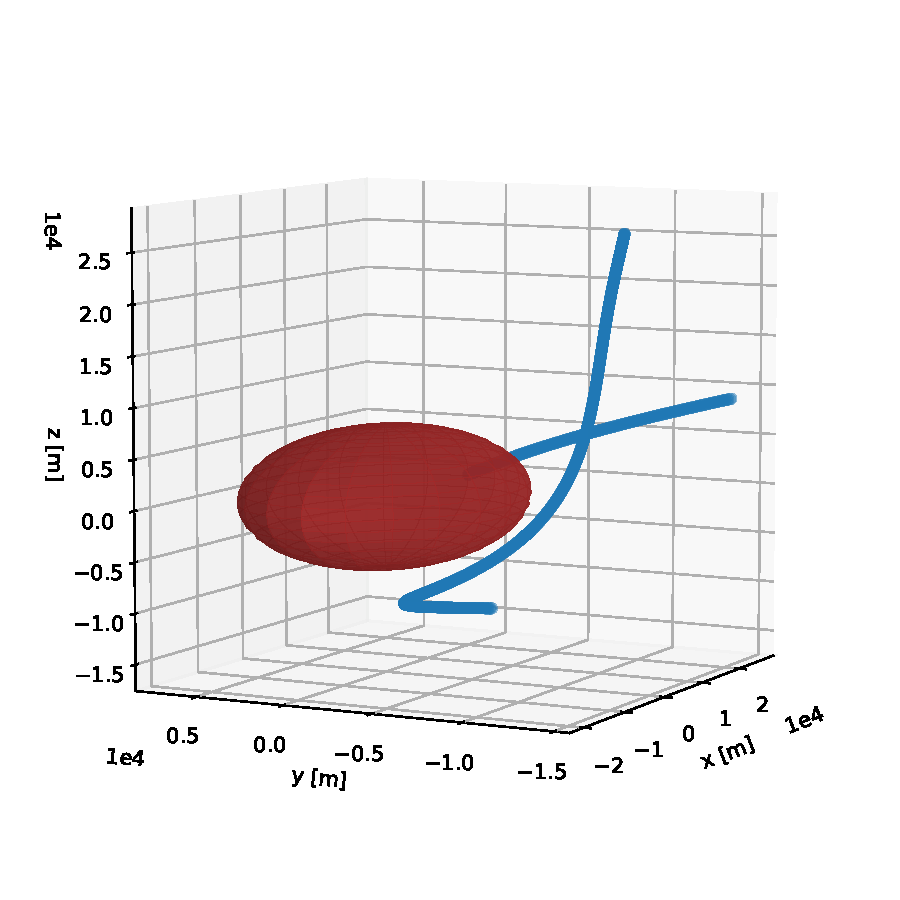
\includegraphics[width=\textwidth, height=0.4\textheight, keepaspectratio=true]{Images/capture_vv_closeProximity3D.pdf}
    \label{fig:capture_vv_3d_plot_1}
}

\subfloat[]{
    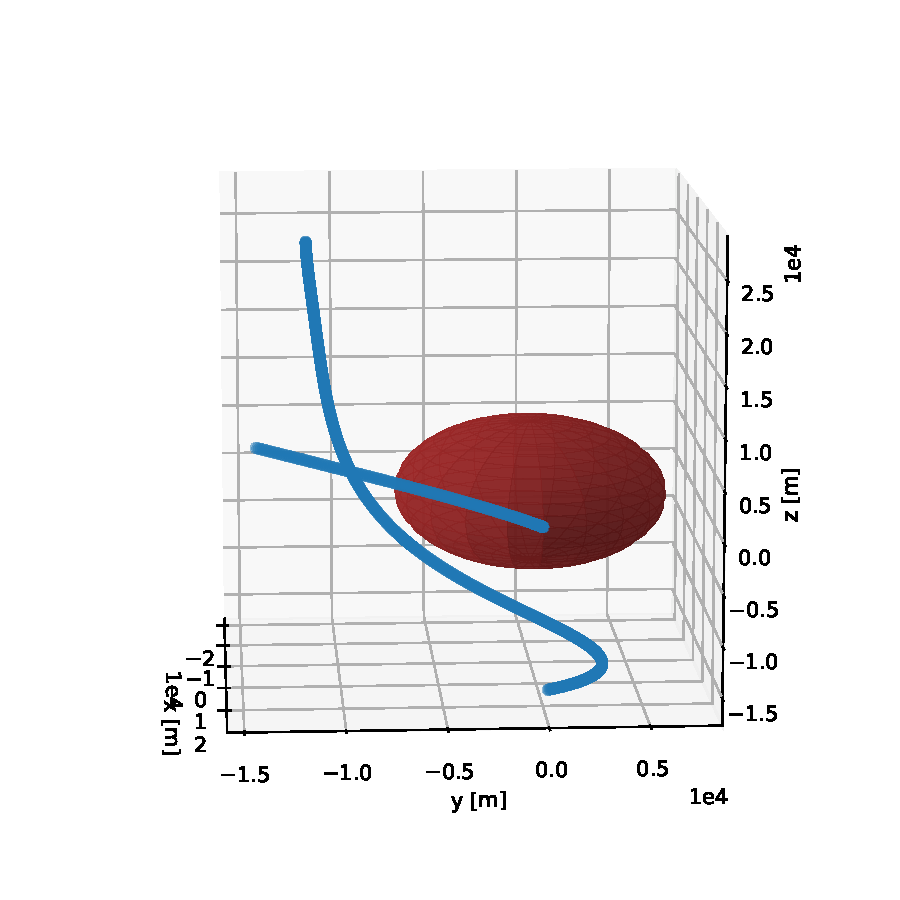
\includegraphics[width=\textwidth, height=0.4\textheight, keepaspectratio=true]{Images/capture_vv_closeProximity3D_frontview.pdf}
    \label{fig:capture_vv_3d_plot_2}
}
\caption{3D trajectory data points for a capture scenario. The data points plotted here are for the case when the particle has a range $\leq 1.5\alpha$, i.e., 1.5 times the largest semi major axis of the asteroid. This check was performed to ensure that the particle has not experienced a re-impact situation that went unnoticed by the simulator.}
\label{fig:capture_vv_3d_plot}
\end{figure}
\FloatBarrier
%%%

\section{Conclusion}
\label{sec:conclusion_vv}
In this chapter, we presented results for verification and validation of the simulator \gls{NAOS}. The tests, and the results from it, proved the authenticity of \gls{NAOS} as we verified its high-level functioning layers such as the perturbing force models, gravity field model, numerical propagator, regolith orbital dynamics, regolith launch parameters and final fate. Validating the aforementioned, in general, validates the functioning of the simulator developed for thesis. However, it must be noted that the high-level validation tests may, often, not act as proofs of correct performance for the lower functional layers of any simulator and hence individual unit tests and sanity checks should be written within the simulator itself to check for bugs that may appear under special circumstances.
%
\newline\newline
%
In this regard, it should be noted that \gls{NAOS} has certain unit test files to validate the lower functional layers using external verified data, for example the cubic root solver for the gravity potential model, the Cartesian to Kepler converter etc. The unit test file is an independent piece of code that checks the performance of, say, the cubic root solver against known data. This unit test file then not only validates its parent function, but also ensures that in future if the parent function is ever modified, then the changes also conform to a correct output value when matched against the same external verified data as before.
%
\newline\newline
%
In addition to this, the code for \gls{NAOS} was developed sequentially and by using modular functions and C++ template files that enable unit testing of several features of the code without changing its parameters manually to accommodate external data. Thus the parent functions are never (manually) hampered to verify its core functionality, otherwise there is always a risk of making an error when changing the code back to its original form. There are several internal sanity checks as well at various points within the \gls{NAOS} code to ensure bugs can be spotted before compromising the integrity of the simulated data. Some of these sanity checks are re-run in the Python codes of \gls{NAOS} that perform data analysis.
